%%%%%%%%%%%%%%%%%%%%%%%%%%%%%%%%%%%%%%%%%%%%%%%%%%%%%%%%%%%%%%%%%%%%%%%%
%    INSTITUTE OF PHYSICS PUBLISHING                                   %
%                                                                      %
%   `Preparing an article for publication in an Institute of Physics   %
%    Publishing journal using LaTeX'                                   %
%                                                                      %
%    LaTeX source code `ioplau2e.tex' used to generate `author         %
%    guidelines', the documentation explaining and demonstrating use   %
%    of the Institute of Physics Publishing LaTeX preprint files       %
%    `iopart.cls, iopart12.clo and iopart10.clo'.                      %
%                                                                      %
%    `ioplau2e.tex' itself uses LaTeX with `iopart.cls'                %
%                                                                      %
%%%%%%%%%%%%%%%%%%%%%%%%%%%%%%%%%%
%
%
% First we have a character check
%
% ! exclamation mark    " double quote  
% # hash                ` opening quote (grave)
% & ampersand           ' closing quote (acute)
% $ dollar              % percent       
% ( open parenthesis    ) close paren.  
% - hyphen              = equals sign
% | vertical bar        ~ tilde         
% @ at sign             _ underscore
% { open curly brace    } close curly   
% [ open square         ] close square bracket
% + plus sign           ; semi-colon    
% * asterisk            : colon
% < open angle bracket  > close angle   
% , comma               . full stop
% ? question mark       / forward slash 
% \ backslash           ^ circumflex
%
% ABCDEFGHIJKLMNOPQRSTUVWXYZ 
% abcdefghijklmnopqrstuvwxyz 
% 1234567890
%
%%%%%%%%%%%%%%%%%%%%%%%%%%%%%%%%%%%%%%%%%%%%%%%%%%%%%%%%%%%%%%%%%%%
%
\documentclass[10pt]{iopart}
\usepackage{latexsym}
\usepackage{graphicx}
\usepackage{iopams}
\usepackage{color}

%\documentclass[12pt]{iopart}
%\newcommand{\gguide}{{\it Preparing graphics for IOP journals}}
%Uncomment next line if AMS fonts required
%\usepackage{iopams}  
%\usepackage {amsmath}
%\usepackage {amssymb}
%\usepackage {amsfonts}
%\usepackage {amsthm}
%\usepackage {mathrsfs}
%\usepackage {natbib}
%\usepackage {latexsym}
%\usepackage {graphicx}
%\usepackage {dsfont}
%\usepackage {times}
%\usepackage {txfonts}
%\usepackage {rotating}
%\usepackage {wasysym}
%\usepackage {multirow}
%\usepackage {hhline}
\usepackage{hyperref}
%\usepackage {color}
\usepackage{bm}
%\usepackage{appendix}
\usepackage{acronym}
%\usepackage{dcolumn}   % needed for some tables
\usepackage{url}
\usepackage[normalem]{ulem}   % temporal one in draft.
\usepackage{xspace}

%\usepackage{harvard}
\usepackage{amsopn} % for using DeclareMathOperator

% variable shortcuts 
\newcommand{\Hub}{H_{0}}
\newcommand{\DL}{D_{\mathrm{L}}}
\newcommand{\lam}{\bm{\lambda}}
%\newcommand{\data}{\bm{d}}
%\newcommand{\sigpar}{\bm{\theta}}
%\newcommand{\nuispar}{\bm{\lambda}}
%\newcommand{\globpar}{\bm{\gamma}}
%\newcommand{\model}{\mathcal{H}}

\newcommand{\curlH}{\mathcal{H}}
\newcommand{\gws}{\tilde{h}}

%% ----- input git-version tag
\input{tag.tex}

\newcommand{\dcc}{LIGO-PXXXXXXXX}
\newcommand{\cm}[1]{\textcolor{red}{CM: #1}}
\newcommand{\MP}[1]{\textcolor{blue}{MP: #1}}
\newcommand{\lw}[1]{\textcolor{green}{LW: #1}}

\DeclareMathOperator{\erf}{erf}

\begin{document}

\title{Astrophysical calibration of gravitational-wave detectors}

\author{L.~Wright$^1$, M.~Pitkin$^1$ \& C.~Messenger$^1$}
\address{$^1$ SUPA, School of Physics and Astronomy, University of
  Glasgow, Glasgow G12 8QQ, United Kingdom}
\eads{\mailto{matthew.pitkin@glasgow.ac.uk}, \mailto{christopher.messenger@glasgow.ac.uk}}

\begin{abstract}
  We present an investigation into the potential of calibrating \MP{change to: ``assessing the validity of the calibration''?}
  gravitational wave detector outputs through the use of standard
  sirens. Such signals, as measured via gravitational wave
  observations provide an estimated luminosity distance which is
  subject to uncertainties in the calibration of the data.  If a host
  galaxy is identified for a given source then its redshift can be
  obtained and combined with current knowledge of the cosmological
  parameters.  This will yield the true luminosity distance and allow
  the direct comparison with the estimated value.  Discrepancies can
  then be used to correct the original calibration.~\cm{Update at end}
\end{abstract}

% acronym definitions
\acrodef{GW}[GW]{gravitational wave}
\acrodef{BNS}[BNS]{binary neutron star}
\acrodef{MWEG}[MWEG]{Milky Way equivalent galaxies}
\acrodef{BBH}[BBH]{binary black hole}
\acrodef{NSBH}[NSBH]{neutron star black hole}
\acrodef{SNR}[SNR]{signal-to-noise ratio}
\acrodef{GRB}[GRB]{gamma-ray burst}
\acrodef{sGRB}[sGRB]{short gamma-ray burst}
\acrodef{CBC}[CBC]{compact binary coalescence}
\acrodef{EM}[EM]{electro-magnetic}

%Uncomment for PACS numbers title message
%\pacs{00.00, 20.00, 42.10}
% Keywords required only for MST, PB, PMB, PM, JOA, JOB? 
%\vspace{2pc}
%\noindent{\it Keywords}: Article preparation, IOP journals
% Uncomment for Submitted to journal title message
%\submitto{\JPA}
% Comment out if separate title page not required
\maketitle

%%%%%%%%%%%%%%%%%%%%%%%%%%%%%%%%%%%%%%%%%%%%%%%%%%
%%%%%%%%%%%%%%%%%%%%%%%%%%%%%%%%%%%%%%%%%%%%%%%%%%
\section{Introduction\label{sec:intro}}

% introduce GWs and BNS systems
It is expected that the advanced generation of interferometric \ac{GW}
detectors will detect waves emitted from $O(10s)$ of compact binary
coalescences.  One such class of these cataclysmic events, the inspiral and
merger of \ac{BNS} systems will be detected out to a maximum range of $\approx
450$ Mpc. Assuming the current best estimates for the cosmological parameters,
this is equivalent to a redshift $z\approx 0.1$. As noted by \cite{1986Natur.323..310S} \ac{CBC}
systems can be used as cosmological distance markers, otherwise known as
``standard sirens'' (analogous to the \ac{EM} standard candles). Standard sirens
allow ...

% BNS systems are GRBs
It is considered likely that the merger of \ac{BNS} systems, in addition to
emitting detectable \acp{GW}, is also the mechanism for producing \acp{sGRB}.
In this scenario these \ac{EM} events are produced through the ... and result
in tightly beamed emission parallel to the orbital angular momentum vector of
the \ac{BNS} system. Additional evidence for the coincidence of \acp{sGRB} with
\ac{GW} events are the estimated astrophysical rates of both phenomena.
Observations of \acp{sGRB} give a rate of XXX Mpc$^{-3}$yr$^{-1}$ which can be
compared to estimates of \ac{BNS} merger rates of XXX-XXX Mpc$^{-3}$yr$^{-1}$.
This latter range is obtained from population synthesis models together with
knowledge of the X known \ac{BNS} systems in our galaxy. 
  
% talk about the calibration idea
If a single \ac{GW} event is observed in coincidence with a \ac{sGRB} it will \MP{may?}
be possible to identify the host galaxy of the \ac{BNS} source.  With this
information a spectroscopic redshift can be very accurately obtained. With
knowledge of the redshift, using current best estimates for the Hubble constant
and other cosmological parameters, the true luminosity distance can be
estimated to $\sim 1\%$ accuracy.  The \ac{GW} measurement acts as a standard
siren also giving us a direct measurement of the luminosity distance to the source.
The accuracy of such a measurement depends on a number of factors including the
accuracy with which the \ac{GW} detector has been calibrated.  Hence comparison
with the distance estimate from the \ac{sGRB} we can re-calibrate (or validate)
the existing experimentally obtained calibration. 

% What do we do in this paper
In this paper we investigate the feasibility of this approach for single
coincident \ac{GW}--\ac{sGRB} events and establish the validation power of such
a calibration technique.  In Sec.~\ref{sec:calibration} we briefly summarize
the existing experimental technique for \ac{GW} detector calibration and its
expected accuracy.  We then review the concept of \ac{GW} standard sirens and
their proposed coincident \ac{EM} signatures, the \acp{sGRB} in
Secs.~\ref{sec:sirens} and~\ref{sec:GRB}. In Sec.~\ref{sec:single} we present
the results of Monte-Carlo simulations for the purpose of luminosity distance
estimation using \ac{GW} events. In Sec.~\ref{sec:cosmo} we show the likely
accuracy of \ac{sGRB} distances obtained from their host galaxy redshift and in
Sec.~\ref{sec:discussion} we conclude.    

%%%%%%%%%%%%%%%%%%%%%%%%%%%%%%%%%%%%%%%%%%%%%%%%%%
%%%%%%%%%%%%%%%%%%%%%%%%%%%%%%%%%%%%%%%%%%%%%%%%%%
\section{Gravitational wave detector calibration\label{sec:calibration}}

\cm{We need to define our model for the calibration, i.e. are we talking
about amplitude only and are we breaking this up over frequency.}

\MP{In this paper I think we stick to just talking about a single overall amplitude calibration scale.}

The technique used throughout GW research in calibrating the detectors is
carried out through a complicated system of physical manipulations of the
Fabret-Perot Michelson interferometer; where an elaborate feedback system is
used to sustain a defined measurement in arm length difference between the
moving mirrors~\cite{LIGOCal}. In general, the interferometers are set to move
at a frequency corresponding to a GW signal. An error signal is then found
through the Pound-Driver-Hall technique~\cite{Black} for mirror stabilisation
which is proportional to the difference in mirror separation of the
Fabret-Perot Michelson interferometer. The Pound-Drever-Hall technique is
essentially a control loop feedback system in which the difference output (in
GW detectors, this is the distance the mirrors move due to the GW) and the the
output set is reduced to the highest degree of certainty. This is just a brief
overview of the calibration method currently used, and is an extensive study in
itself, see \cite{Vitale:2012} and references therein. For advanced LIGO and Virgo,
at the frequency range used in this project, the error in the calibration using
the `hardware injection method' is roughly $10\%$ \cite{Vitale:2012}. This is a
benchmark set for the error estimation using the proposed new method in this
project.~\cm{Clean this up and expand.}

% Describe our model for the calibration
\MP{The gravitational wave strain is measured through the differential arm length, $\Delta L$, changes
of the interferometer via $h = \Delta L(f) / L$, where $L$ is the full arm length.
Calibration is required to relate the actual measured interferometer error signal output
$e(f)$ to $\Delta L$. This relation is known as the length response function, $R(f,t)$,
defined such that
\begin{equation}
\Delta L(f) = R(f,t) e(f),
\end{equation}
where $R$ varies slowly in time (in comparison to transient signal timescales).
Calculation of $R$ requires the measurement of various functions within a control feedback loop
(see \cite{Vitale:2012} for a brief overview of this), which are subject to
uncertainties. In this study we will assume an estimate of $R$ is available (although
in theory we could take on the role of estimating $R$ itself), but that it differs from the
truth through some unknown scale factor, $s$, so that
\begin{equation}
h(f) = s h_{\rm m}(f) = s \frac{R(f,t) e(f)}{L},
\end{equation}
where $h(f)$ is the true strain and $h_{\rm m}(f)$ is the measured strain.
In this analysis we will simplify the situation by assuming that $s$ is a constant with
respect to frequency, but in future studies that assumption could be dropped and $s$
could take some functional form, or piece-wise fit, with respect to $f$.}

%%%%%%%%%%%%%%%%%%%%%%%%%%%%%%%%%%%%%%%%%%%%%%%%%%
%%%%%%%%%%%%%%%%%%%%%%%%%%%%%%%%%%%%%%%%%%%%%%%%%%
\section{Binary neutron star standard sirens\label{sec:sirens}}

We should explain what this means starting with reference
to~\cite{1986Natur.323..310S}.

%%%%%%%%%%%%%%%%%%%%%%%%%%%%%%%%%%%%%%%%%%%%%%%%%%
%%%%%%%%%%%%%%%%%%%%%%%%%%%%%%%%%%%%%%%%%%%%%%%%%%
\section{GRB counterparts\label{sec:GRB}}

% what are sGRBs 
\cm{What are sGRBs?}\\

% discuss joint-event rates
\cm{Discuss the expected rate of joint detections}\\

% observing a coincident event
The most likely scenario in which a coincident \ac{GW}--\ac{sGRB} event would
be identified is through the targeted follow-up of an observed \ac{sGRB} or by
post-facto matching of \ac{GW} trigger lists with known \ac{sGRB} events.  The
likelihood of being able to follow-up \ac{GW} events using gamma-ray telescopes
with low enough latency to catch a \ac{sGRB} is low.  Compounding this issue is
the relatively large \ac{GW} sky error-box giving a field-of-view for the
\ac{EM} observatories to search spanning $\sim 100$'s of square
degrees~\cite{grb}.  For the \ac{GW} follow-up of \ac{sGRB} scenario the merger
time for \ac{BNS} systems will be estimated from the \ac{sGRB} to within a few
seconds~\cite{grb}.  This makes the follow-up search less computationally
expensive since it is performed over a smaller range of data using potentially
fewer numbers of waveform templates.  This computational saving enables the use
of a more computationally expensive multi-detector coherent scheme rather than
the cheaper coincidence methods used in the untargeted searches. 

% discuss the inclination angle issue
A fortunate consequence of a joint \ac{GW}--\ac{sGRB} observation will be the
fact that in order for such an event to be observed, the \ac{BNS} system must
have had its orbital angular momentum vector pointing towards (or away) from
the detector.  The actual inclination angle of the system, defined as the angle
between the orbital angular momentum vector and the line of sight, must be $<$
half of the \ac{sGRB} beaming angle.  This prerequisite property limits us to
systems that are approximately ``face-on'' and therefore biases us to higher
\ac{SNR} signals.  However, as discussed earlier, the property of beaming
severely impacts the probable rate of such joint observations.   


%%%%%%%%%%%%%%%%%%%%%%%%%%%%%%%%%%%%%%%%%%%%%%%%%%
%%%%%%%%%%%%%%%%%%%%%%%%%%%%%%%%%%%%%%%%%%%%%%%%%%
\section{Analysis}

\cm{This should be the simplest case we can do.  We need to cut a lot of this.}

\MP{We want to assess how well a calibration scale factor can be estimated
from a single observed \ac{GW} associated with a particular \ac{sGRB}. As we {\it a priori}
have no knowledge of the likely location and distance of such an event we have performed
simulations of multiple events to see the expected distribution the accuracy of the
calibration scale factor recovery.}

% Describe what we are going to do in this section
Let us consider a single \ac{GW} detection of the inspiral stage of a \ac{BNS}
merger and assume that this signal has been associated with a potential
\ac{sGRB} detection. We therefore also assume that the inclination angle
of the binary is consistent with a given \ac{sGRB} beaming angle.  Finally we
assume that a host galaxy has been identified for the source and that the sky
position is therefore known to high precision.

\MP{We perform 100 simulations at each of a range of distances from 10\,Mpc out
to 200\,Mpc. For the simulations at each distance range we have allowed the
source's sky position to be randomly drawn from a uniform distribution over
the sky, the polarisation angle $\psi$ to drawn from a uniform distribution in the
range $[0, \pi/2]$, the coalescence phase to be drawn from a uniform distribution
in the range $[0, 2\pi]$, and the inclination angle drawn from a Gaussian with range XX?.
The binary system masses have been fixed as $1.4\,{\rm M}_\odot$ (based on the
very good assumption that whatever masses are chosen in these cases they will be
recovered to high accuracy) and the time of coalescence is fixed.}
 
% Describe the signal model (Taylor F2 etc...)
We use the post-Newtonian Taylor F2 waveform approximation for modelling the
signal whereby the \ac{GW} phase for 2 point-particles of mass $m_{1}$ and
$m_{2}$ is given by
%
\begin{equation}
\label{eq:gwphase}
  \Psi(f) = 2\pi f t_\mathrm{c} - \phi_{\mathrm{c}} - \frac{\pi}{4} +
\frac{3}{128\eta\nu^{5}}\sum\limits_{k=0}^{7}\alpha_{k}\nu^{k}.
\end{equation}
%
Here $\eta=m_{1}m_{2}/M^{2}$ is the symmetric mass-ratio with $M=m_{1}+m_{2}$
the total mass.  The post-Newtonian expansion parameter is $\nu=(\pi M
f)^{1/3}$ and the coefficients are $\alpha$.

The frequency-domain polarisation amplitudes are then defined as
%
\begin{eqnarray}\label{eq:signal}
  \gws_{+}(f) &=& \frac{1+\cos^{2}\iota}{2D_{L}}
\frac{\mathcal{M}^{5/6}}{\pi^{2/3}}
\sqrt{\frac{5}{24}}f^{-7/6}e^{-i\Psi(f)} \nonumber \\
  \gws_{\times}(f) &=&
 i\frac{\cos^{2}\iota}{D_{L}}\frac{\mathcal{M}^{5/6}}{\pi^{2/3}}
\sqrt{\frac{5}{24}}f^{-7/6}e^{-i\Psi(f)}
\end{eqnarray}
%
where the chirp-mass $\mathcal{M}$ is defined as $\mathcal{M}=M\eta^{3/5}$,
and $\iota$ is the inclination angle.  The \ac{GW} strain measured
at the $k$'th detector is then given by
%
\begin{equation}
  \label{eq:gravsig}
   \gws^{k}(f) = \big[ F_{+}^{k}(\alpha, \delta, \psi)\gws_{+}(f) +
F_{\times}^D(\alpha, \delta, \psi)\gws_{\times}(f)\big]
\end{equation}
%
where $F_{+},F_{\times}$ are the antenna response functions which are dependent
upon the polarisation angle $\psi$ and the sky position of the source
$\alpha,\delta$.

% Define the detectors and the noise epoch we will be using
For this analysis we will consider advanced generation instruments operating
at their design sensitivity, \MP{with noise power spectral densities taken from
\cite{2013arXiv1304.0670L}}. The network we consider is the 3 detector H1--L1--V1 configuration. 

% Define the likelihood function we will be using
We consider that the measured data in any detector is defined as
%
\begin{equation}
  \tilde{d}_{k}(f)=\tilde{n}_{k}(f)+s\gws_{k}(f,\btheta)
\end{equation}
%
where $\tilde{n}(f)$ is the Fourier transform of Gaussian noise drawn from a
distribution consistent with the power-spectral-density of the advanced
detector noise. 

\subsection{Method}

\MP{Our aim is to estimate the marginal posterior probability distribution function (pdf)
for the unknown calibration scale factor. We use Bayes' theorem for which we need to define
a likelihood function and prior pdfs on the signal parameters being estimated. In this
analysis we use the Markov chain Monte Carlo code {\tt emcee} \cite{2013PASP..125..306F} to sample 
the posterior distribution.} We use a Gaussian likelihood function given by
%
%\begin{equation}
%  p(\vec{d} | \vec{\theta}, \curlH, I) \propto \exp\Bigg[ 2\Delta
%f\sum_{k>0}\frac{|\tilde{d}(f_{k}) - \tilde{h}(f_{k})|^{2}}{S(f_{k})}\Bigg]
%\end{equation}
\begin{equation}
\fl p(\bi{d} | \btheta, \curlH, I) \propto \exp{\left[4\Delta f \sum_{k=1}^{N_{\rm det}}
  \sum_{i=i_{f_{\rm low}}}^{i_{f_{\rm high}}}\frac{\Re{\left\{ \tilde{d}^{*}_{k,i} 
\gws_{k,i}(\btheta) - \frac{1}{2}\left(\gws^*_{k,i}(\btheta)\gws_{k,i}(\btheta) + 
\tilde{d}^*_{k,i}\tilde{d}_{k,i}\right) \right\}}}{S_{k,i}}\right]}
\end{equation}
% 
where $\Delta f$ is the frequency resolution of the data, $S_k$ is the $k^{\rm th}$ detector's one 
sided noise power spectral density, and the $i$ indices increment over frequency with $i_{f_{\rm 
low}}$ and $i_{f_{\rm high}}$ corresponding to the lower and upper range in frequencies used for 
our analysis (which were 40\,Hz to 1600\,Hz respectively \MP{Should we actually go down to 20\,Hz -- 
I imagine for BNS systems it doesn't make much difference?}). The source parameters, and the 
unknown scale factor, have been subsumed into a vector $\vec{\theta}$. For a network of detectors, 
the overall likelihood function becomes a product of the likelihoods for each detectors, i.e.\
\begin{equation}
  \label{eq:mult-likeli}
  p(\bi{d}| \btheta, \curlH) = \prod \limits_D p(\bi{d}^D| \vec{\theta}, \curlH)
\end{equation}
where $D = \{H,L,V\}$.

% describe what parameters we will be considering and their priors
We assume uniform prior distributions on the unknown nuisance parameters
$\phi_{\mathrm{c}},\psi$ on the ranges $[0, 2\pi]$ and $[0, \pi/2]$ respectively.
The time of coalescence is
restricted to a prior range of $\pm 10$ msec around the true value.  Given our
assumption of an \ac{sGRB} counterpart and host galaxy, we treat the sky
position as exactly known. We also consider the cosine of the inclination angle to be drawn
from a zero-mean Gaussian with standard deviation $0.1$ consistent with an
uncertainty on \ac{sGRB} opening of XXX~\cm{What was exactly done here?}.  The
main parameter of interest, the calibration scale factor $s$ is assumed to have
a uniform prior distribution on the range $(0,2)$.    

\subsubsection{Prior ranges}\label{sec:priors}

The primary reason why we can use coincident observations with a GRB as a potential check of 
detector calibration is that the GRB allows us to constrain our priors on various parameters that 
would normally be highly correlated with the signal amplitude. The most important of these is that 
the GRB can provide a very tight constraint on the source distance\footnote{A consequence of our 
choice of BNS signals is that they will only be observable within the local Universe ($z \sim 
0.1$), so the relation between the measured GRB redshift and distance is simple and is negligably 
effected by the choice of cosmology.}. In this analysis we therefore assume that the source distance 
is known (i.e.\ has a $\delta$-function prior). Another piece of information that we can use from 
having a coincident GRB is that the system must be close to face-on, which allows us to place prior 
constraints on the system inclination angle. In our analysis we take two scenarios: the first use a 
prior on the beam opening angle (half-width of the beam) with a Gaussian distribution with zero mean 
and $\sigma = 5^{\circ}$, whilst the second uses $\sigma = 20^{\circ}$. Beam opening angles for 
short GRBs are relatively poorly constrained as they are based on only a few jet break detection, 
however \cite{2014ApJ...780..118F} give a median opening angle value of $\sim 10^{\circ}$. If we 
assume that the beam opening angle is a half-normal distribution, for which the median is given by 
$\sqrt{2}\erf{}^{-1}(1/2)\sigma \sim 0.67\sigma$, then a median of $\sim 10^{\circ}$ corresponds to 
$\sigma \sim 14.8^{\circ}$.

As we have assumed that the GRB progenitor is a binary neutron star system the prior we use for the 
system component masses is a Gaussian distribution for both components with means 
of $1.35\,\textrm{M}_{\odot}$ and standard deviations of $0.13\,\textrm{M}_{\odot}$ 
\MP{(reference)}. In reality, for all the systems we use in our study, the chirp mass, which 
we see from equation~\ref{eq:signal} plays a role in the overall signal amplitude, is very well 
constrained by the systems phase evolution, so our prior could be expanded with minimal effect on 
the results. In the future neutron star-black hole systems could be included, although this add the 
complication of having to include the black hole spin (by using BNS systems we have assumed that 
the spins are small enough that they will introduce only a negligible effect).

The final important piece of information that we can make use of from the GRB observation is the 
sky position of the source, which we take to be known precisely.

For the time of coalescence we use a uniform prior of spanning $\pm0.01$\,seconds around the 
recorded time of the signal that would be returned by the detection pipeline. For the reference 
phase a uniform prior between 0 and $2\pi$ is used, and for the polarisation angle a uniform prior 
between 0 and $\pi/2$ is used. As the signals we use are generally close to being circularly 
polarised (face-on) the phase and polarisation angle will be degenerate meaning the exact 
combination of them will have very little effect of the result.

Finally, we require a prior on the calibration scale factors for each detector. We make the 
assumption that in general the calibration will be correct, so want to use a prior that is peaked 
at unity. We also assume that the probability density that the calibration scale factor is either 
larger or smaller than unity by an equivalent factor, e.g.\ $s=10$ or $s=0.1$, is the same. For this 
we therefore use a log-normal distribution as our prior
\begin{equation}
 p(s|I) = \frac{1}{s\sigma\sqrt{2\pi}}\exp{\left( -\frac{(\ln{s} - \mu)^2}{2\sigma^2} \right)},
\end{equation}
where we chose $\sigma = 1$, which in turn means that having the mode at unity gives $\mu = 1$. 
With these parameters the prior probability density at 0.1 and 10 is $\sim 1/14$ of that at 1. 
Note that this prior does not provide produce a symmetric amount of probability about unity, but 
given our simulation criterion described below in Section~\ref{sec:simulations} we find that the 
likelihood generally overwhelms the prior. As $s$ is a scale factor we also have the further 
constraint that it must be positive.

\subsection{Simulations}\label{sec:simulations}

To estimate how well we can constrain the calibration scaling each detector in an advanced 
detector network we have performed simulations with injected BNS signals at a range of distances 
(50\,Mpc to 450\,Mpc on 50\,Mpc increments). The simulations use the two Advanced LIGO detectors 
(one at Hanford -- H1 -- and one at Livingston -- L1) and the Advanced Virgo detector (V1). We 
assume all are expected to be operating at their design sensitivity.

% Describe the ensemble of simulations used
As described in Section~\ref{sec:priors} we had two different scenarios for the prior distribution 
of source system inclination angles, so we have produced separate simulations for both cases. In 
each case 1000 sources were created with distributions on the inclination, component masses,
reference phase and polarisation angle drawn from their respective prior distributions. For the 
time of coalescence the times were held fixed within the centre of the prior window. When drawing 
the sky position points were drawn uniformly over the sky. However, with all these an additional 
constraint was imposed based on the fact that we require a distributions sources that could 
actually have been detected. We therefore include the requirement from \cite{2012PhRvD..85h2002A} 
that their be at least two detectors in the network for which the SNR is $\gtrsim 5.5$ (as these 
would be signals coincident with a GRB we do not include the often used further constraint that 
the total coherent network SNR is greater than 12). This generally means that as we go to larger
distances our population of sources that fulfil this criterion will not be uniformly distributed
over the sky, and will generally be closer to being circularly polarised.

For each source we applied a fixed calibration scale factor of 1.2, 0.8 and 1.3 for H1, L1 and V1 
respectively.

These simulations allow us to assess how well on average we would be able to constrain the 
calibration scale for a given CBC-GRB coincidence.



\section{Results}\label{sec:results}

For each of the simulated sources we have calculated the 68\% credible region on the scale factors 
for each detector (for a Gaussian distribution this is equivalent to the region bounded by 
$1\sigma$ intervals). For all the signals in each distance increment we have produced the 
distribution of the half widths (i.e.\ $1\sigma$) of these scale factors. These are shown in 
figures~\ref{fig:narrowdist} and \ref{fig:widedist} for the case with the inclination distribution 
with a width of $5^{\circ}$ and $20^{\circ}$ respectively.

\begin{figure}
 \begin{center}
  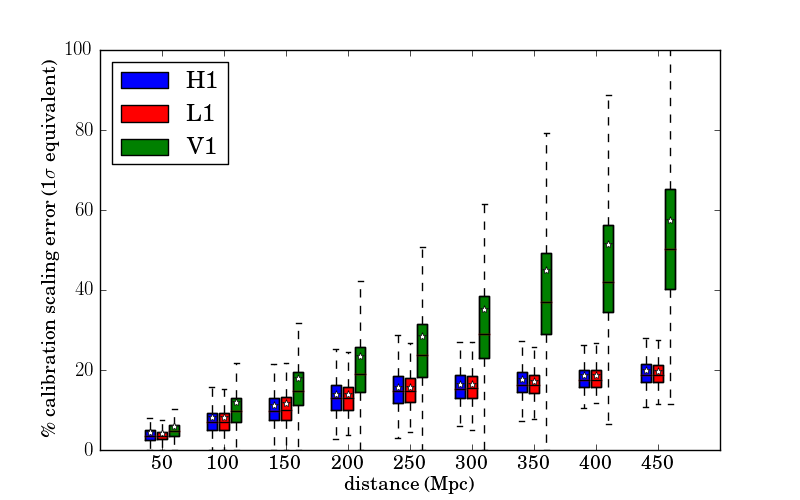
\includegraphics[width=1.0\textwidth]{scale_factors_5degs_boxplot.png}
 \end{center}
 \caption{\label{fig:narrowdist} Add caption!}
\end{figure}

\begin{figure}
 \begin{center}
  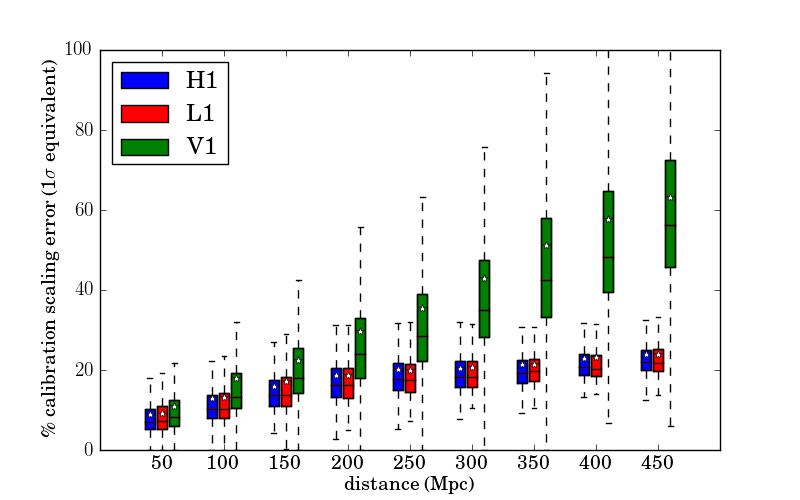
\includegraphics[width=1.0\textwidth]{scale_factors_20degs_boxplot.png}
 \end{center}
 \caption{\label{fig:widedist} Add caption!}
\end{figure}


%%%%%%%%%%%%%%%%%%%%%%%%%%%%%%%%%%%%%%%%%%%%%%%%%%
%%%%%%%%%%%%%%%%%%%%%%%%%%%%%%%%%%%%%%%%%%%%%%%%%%
\section{Distance estimates from \acp{sGRB}\label{sec:cosmo}}

~\cm{Describe the cosmological analysis used to obtain the distance from the
GRB}

%%%%%%%%%%%%%%%%%%%%%%%%%%%%%%%%%%%%%%%%%%%%%%%%%%
%%%%%%%%%%%%%%%%%%%%%%%%%%%%%%%%%%%%%%%%%%%%%%%%%%
\section{Multiple events without counterpart\label{sec:multiple}}

\cm{A discussion of the issues regarding multiple events
without EM counterparts.}

%%%%%%%%%%%%%%%%%%%%%%%%%%%%%%%%%%%%%%%%%%%%%%%%%%
%%%%%%%%%%%%%%%%%%%%%%%%%%%%%%%%%%%%%%%%%%%%%%%%%%
\section{Discussion\label{sec:discussion}}

\cm{What did we learn.}

This paper has shown that for differing levels of SNR, the error in the
calibration is resolved within a certain accuracy range. Initial simulations
used a bad sky position, resulting a low SNR which created larger uncertainty
in resolving $s$. It was shown that for this sky position, the calibration
scale factor estimation was recovered with an accuracy of roughly a $27\%$ for
$D_{L} = 200\,Mpc$ for LIGO Hanford. The resolution of $s$ for a network of
detectors was also shown.

The main results obtained in this project were from analysing randomly chosen
sky positions from the entire field of view for the detector. Through these
simulations, it was shown that this new method of calibration can reach and
surpass the current method in terms of accuracy. The results in
figure~\ref{fig:std-rndsp} show that for half of the randomly chosen sky
positions relate to an estimation of $s$ within a range comparable with the
current methods.

These results are reassuring for parameter estimation of the defining GW signal
and would help in reducing the uncertainty in a direct detection. This project
was; however, time constrained. There are many, many things that could be done
with this project. A true noise realisation with each frequency bin having a
random Gaussian noise would be the next step in calibration error estimation.

This project is only the beginning in testing this new method of calibration.
More rigorous testing has to be carried out for a number of different systems.
As mentioned above, a larger number of random sky positions have to be analysed
to give better understanding of the resolution capabilities of the method. The
current technique of calibration defines the error in the detector to be a
complex function of frequency and phase of the GW. Instead of the simple scale
factor used so far, a more realistic error can be tested to ensure that the
estimation in its value is still comparable with current methods.


For applications of this calibration method, hypothesis testing could be
carried out. Testing different hypothesis is the technique used in determining
a GW signal in a data-set when compared to a noise-only data-set. Being able to
show with confidence that the data contains a signal is the primary focus of GW
research at the moment. Therefore if uncertainty can be removed from the
analysis this will ensure a more confident detection. Using this new method is
resolving and removing the uncertainty is an area which has to be explored.

\MP{We emphasise that our work has assumed that the PSD used in the likelihood function
when estimating the calibration scale factor is an accurate representation of the
PSD at the time of the observed CBC signal. In reality the PSD may be estimated from
a period close to, but not overlapping, the signal time and therefore may be slightly
different \cite{2013PhRvD..88h4044L}. Our result would therefore be completely correlated
with any uncertainty in the PSD estimate, but would still offer an upper limit
on the calibration uncertainty.}

\MP{The BayesLine algorithm \cite{2015PhRvD..91h4034L} may provide a natural
way to perform this analysis in particular when accounting for a frequency
dependent calibration.}

\ack

We would like to acknowledge the useful discussions with a whole bunch
of people. LW was part funded for this work through a Royal Astronomical
Society Undergraduate Research Bursary.
MP is funded by the STFC under grant number ST/L000946/1.

\section*{References}

%\biaxbliographystyle{jphysicsB}
\bibliographystyle{iopart-num}
\bibliography{masterbib}
\end{document}


